\chapter{Proposed Methodology and System Design}\label{proposed}
A novel framework for insider threat detection that combines causal analysis + MAD-based feature refinement + SMOTE + LNNs is proposed which aims to effectively identify hidden behavioral patterns and respond to changes in user activity within an organization from user activity logs. 

\begin{figure}[!ht]
\centering
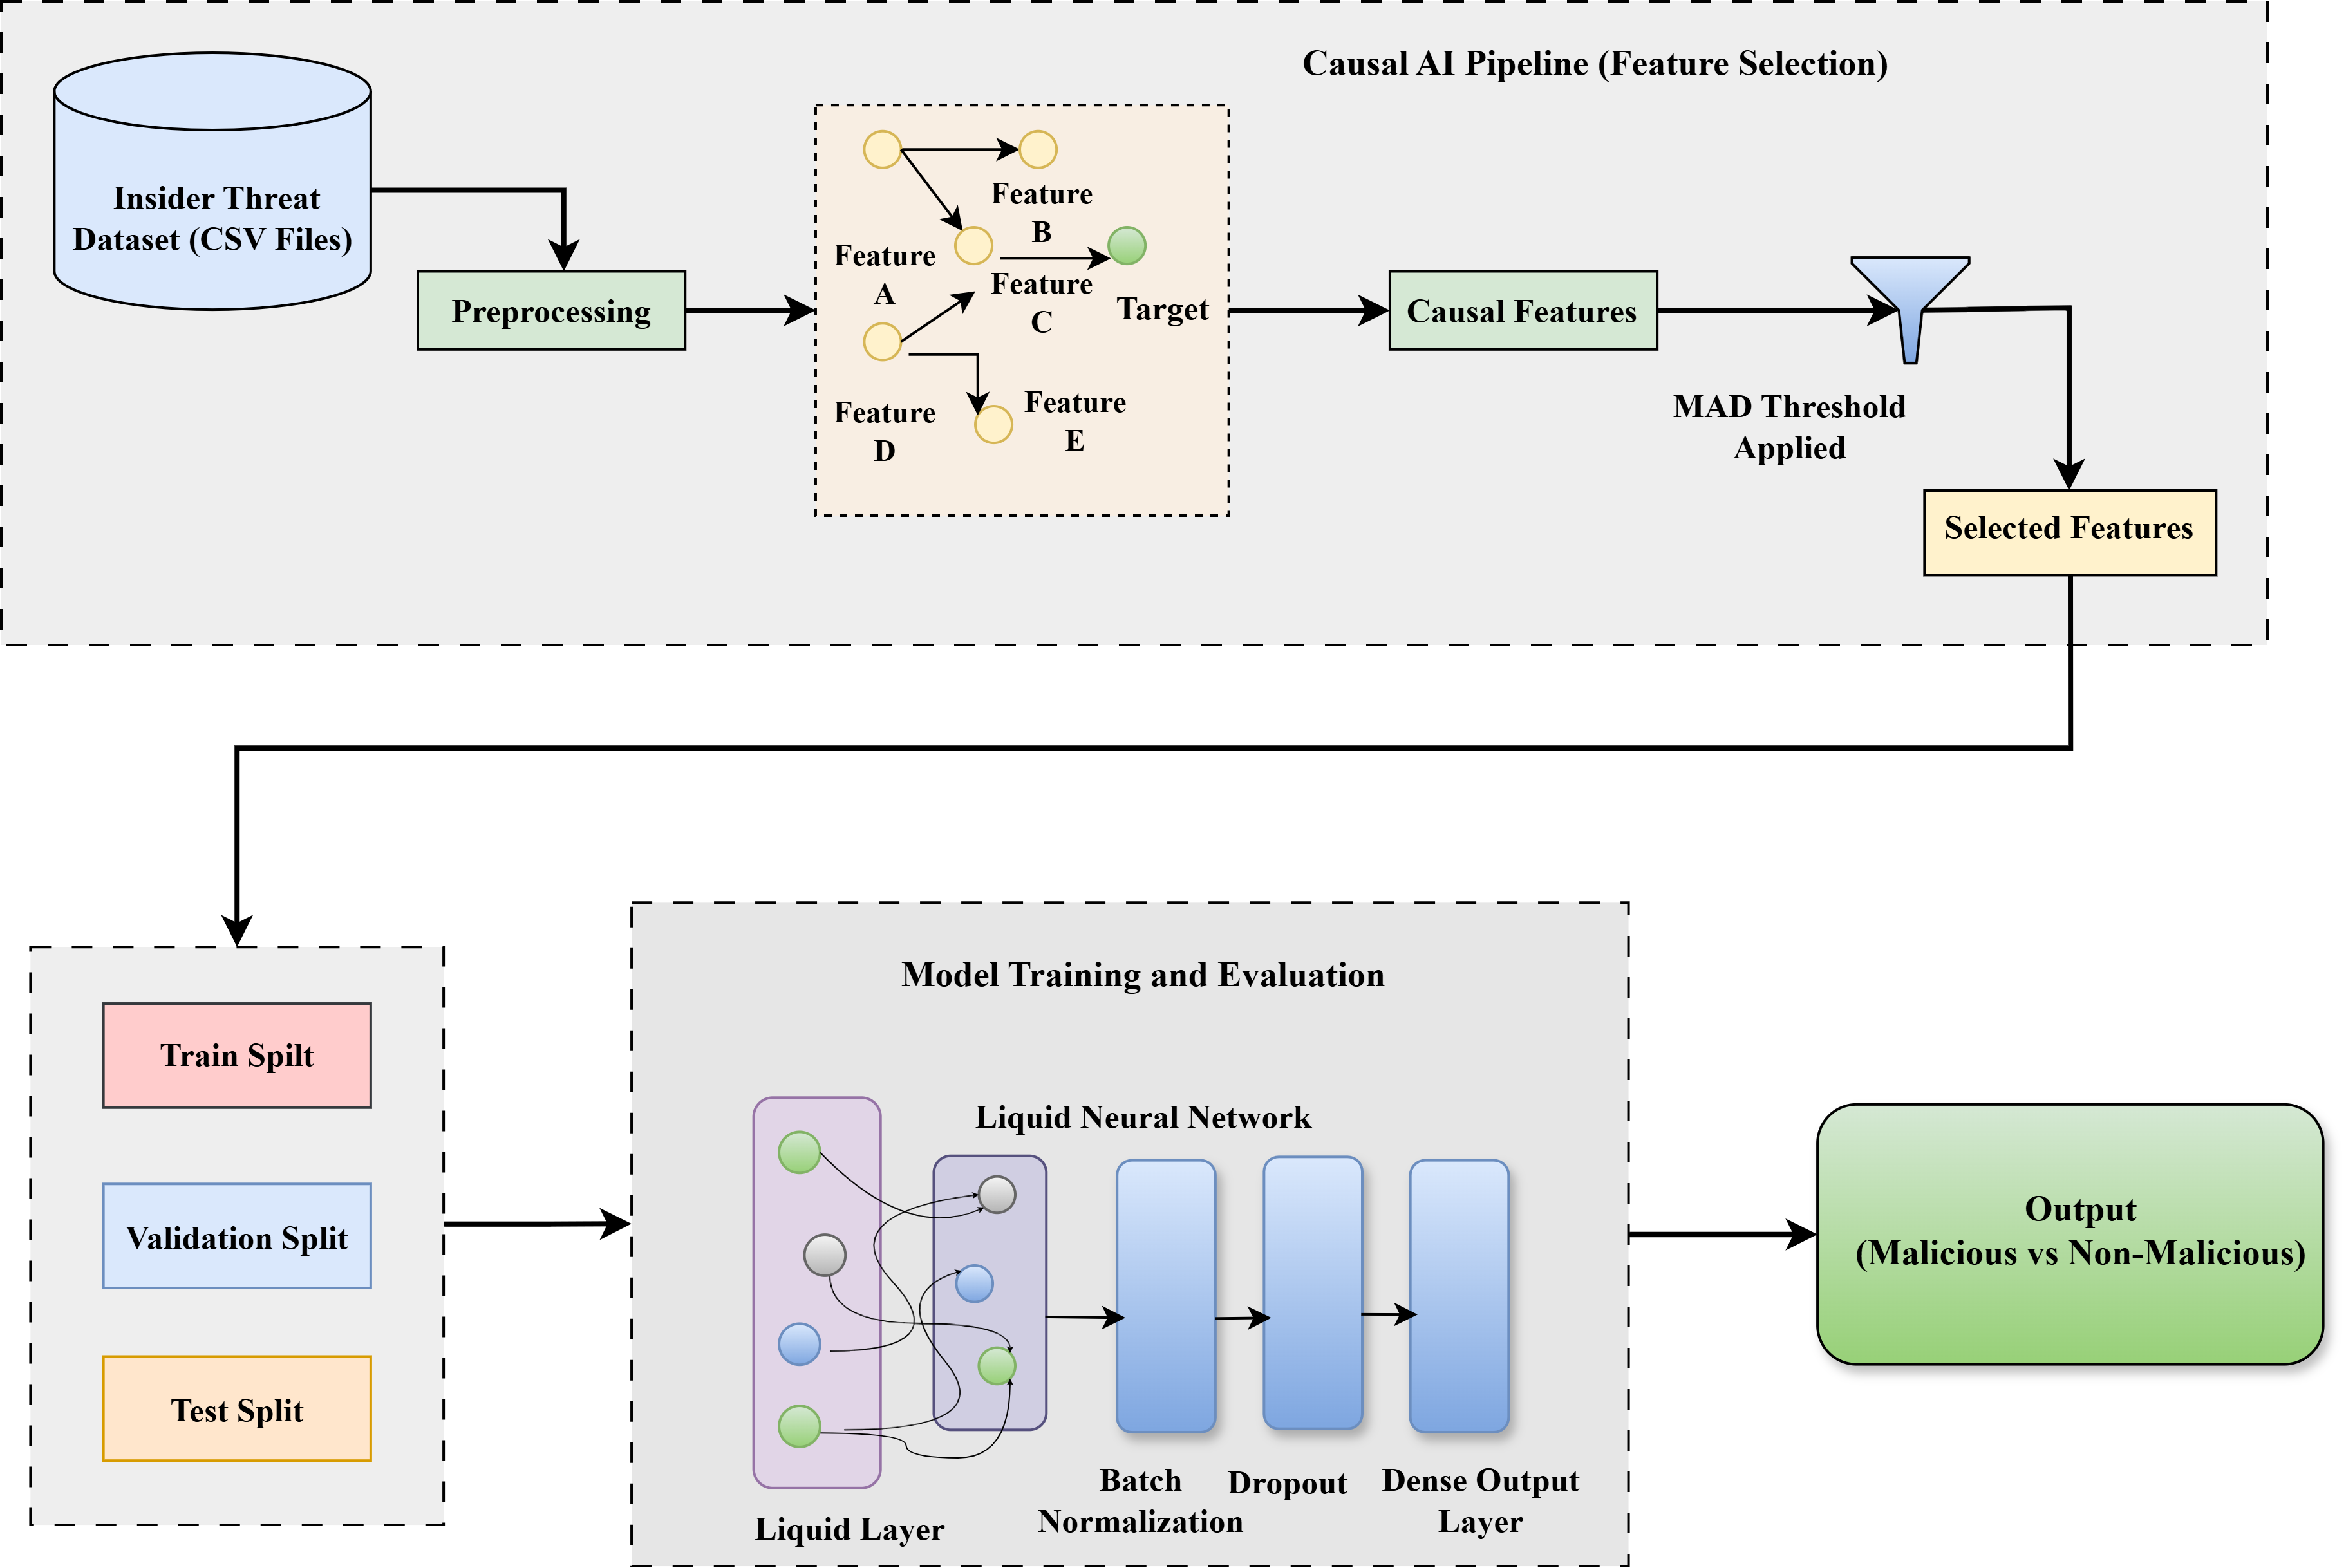
\includegraphics[width=0.95\textwidth,height=0.65\textwidth]{figures/Causal_LNN_1_.png}
\caption{Architecture of the Proposed Method}\label{fig1}
\end{figure}

Figure \ref{fig1} illustrates the proposed architecture, which begins with the collection of insider threat dataset files in  Comma Separated Values (CSV) format, which are then preprocessed. The preprocessed data is then subjected to feature selection through a Causal inference pipeline that performs relationships between features and the target variable. The causal features are filtered with a MAD threshold to select the most useful ones. These features are then divided into training, test, and validation sets. SMOTE is applied on train data for balancing both target classes. The central model is an LNN that handles the data with layers of batch normalization, dropout, and a dense output layer. Lastly, the model outputs whether the input was malicious or non-malicious behavior.





\subsection{Dataset}
The CERTr4.2 dataset is a well-known dataset from CMU for insider threat detection. It simulates real-world workplace activities, including both normal and malicious behavior. The dataset contains user activity logs such as file access, emails, logins, and website visits, which provide insights into employee behavior. It also has psychometric features that measure personality traits, state of mind, and behavioral habits. These features help us understand the psychological factors which can lead to insider behavior.  From both a technical and psychological point of view, each file gives us useful information about how users act. 
\begin{algorithm}
\caption{Insider Threat Detection via Causal Feature Selection and LNNs}\label{alg2}
\DontPrintSemicolon
\LinesNumbered
\small
\KwInput{CERT r4.2 Dataset $\mathcal{D}$ with $n$ samples and $m$ features}
\KwOutput{Classification metrics and confusion matrix}

\vspace{0.3cm}
\textbf{Step 1: Preprocessing (refer Algorithm~\ref{alg1})} \\
\Indp
Apply Session-wise, Day-wise, or Behavior-wise Preprocessing to $\mathcal{D}$\;
Obtain preprocessed feature matrix $X \in \mathbb{R}^{n \times m}$ and label vector $y \in \{0,1\}^n$\;
\Indm

\vspace{0.2cm}
\textbf{Def} \text{CausalFeatureSelection}$(X, y)$:\ \\
\Indp \ForEach{feature $f$ in $X$}{
    Estimate causal effect of $f$ on $y$ using DoWhy\;
}
Apply MAD threshold to select important features\;
\Indm \Return{$X_{sel} \in \mathbb{R}^{n \times m'}$}

\vspace{0.2cm}
\textbf{Def} \text{DataSplitBalanceStandardize}$(X_{sel}, y)$:\ \\
\Indp
Split $(X_{\text{sel}}, y)$ into train/val/test (70/15/15, stratified)\;
Apply SMOTE to training set\;
Reshape $X_{train}, X_{val}, X_{test}$ to $\mathbb{R}^{n \times T \times d}$ format\;
\Indm \Return{$X_{train}, y_{train}, X_{val}, y_{val}, X_{test}, y_{test}$}

\vspace{0.2cm}
\textbf{Def} \text{TrainLNN}$(X_{\text{train}},\ y_{\text{train}},\ X_{\text{val}},\ y_{\text{val}})$:\ \\
\Indp
for LNN Training (\textbf{refer to Algorithm \ref{algo2}) } \\
\Indm \Return{Trained method $f_{\text{LNN}}$}

\vspace{0.2cm}
\textbf{Def} \text{Evaluatemethod}$(f_{\text{LNN}}, X_{test}, y_{test})$:\ \\
\Indp Predict $\hat{y} \gets f_{\text{LNN}}(X_{test})$\;
Compute performance metrics \;
\Indm \Return{Evaluation report}

\vspace{0.2cm}
\textbf{Function} \text{Main()}:\ \\
\Indp $X, y \gets \text{LoadData}(\mathcal{D})$\;
$X_{sel} \gets \text{CausalFeatureSelection}(X, y)$\;
$X_{train}, y_{train}, X_{val}, y_{val}, X_{test}, y_{test} \gets \text{DataSplitBalanceStandardize}(X_{sel}, y)$\;
$f_{\text{LNN}} \gets \text{TrainLNN}(X_{train}, y_{train}, X_{val}, y_{val})$\;
$\text{metrics} \gets \text{Evaluatemethod}(f_{\text{LNN}}, X_{test}, y_{test})$\;
\Indm \Return{Final metrics and evaluation report}
\end{algorithm}
 The CERTr4.2 dataset is used, and data is preprocessed using three different methods: Session-wise, Day-wise, and Behavior-wise Preprocessing representations, which are explained in Algorithm \ref{alg2}.  These preprocessing methods find important patterns in temporal activity, which helps the method tell the difference between normal and bad behavior.
 
\begin{enumerate}

\item  logon.csv – keeps track of when users log in and out of the system.
\item device.csv – keeps track of how external storage devices, like USB drives, are used.
\item email.csv – keeps track of the emails that users send and receive.
\item file.csv – keeps track of how files are accessed and changed.
\item http.csv—has information about how users browse the web.
\item psychometric.csv – score of users' personalities and actions.
\item ldap.csv – keeps track of changes to user roles and the structure of the organization.
\end{enumerate}





\begin{table}[!ht]
\centering
\caption{Overview of CMU-CERTr4.2 dataset}\label{tab5}%
\begin{tabular}{@{}ll@{}}
\toprule
    \textbf{CMU-CERTr4.2 Dataset} & \textbf{Number of Records}  \\
\midrule
Data Collection Period	& 17 months\\
Total Number of Users	& 1,000 Users\\
User Distribution	& 930 Non-malicious, 70 Malicious\\
Logon.csv	& 58,45,859\\
Email.csv	& 26,29,979\\
File.csv	& 44,55,581\\
Device.csv	& 4,05,380\\
Http.csv	& 2,84,34,423\\
Psychometric.csv & 1000 \\
Total Event Count	& 3,27,70,222\\
\bottomrule
\end{tabular}
\end{table}

Table \ref{tab5} shows that the synthetic dataset has been collected over a period of 500 days. Around 1000 user log files have been recorded and of which 70 were insiders. It includes three scenarios of insider threats which are described as follows: \\
\textbf{Scenario 1:}  Suspicious activity: Unsual working patterns of employees are recorded after or before office hours.\\
\textbf{Scenario 2:}  Job-Hunting Data Theft: An employee looking for a new job uses a thumb drive more often to steal data before quitting.\\ \textbf{Scenario 3:} Unauthorized Access and Sabotage: A user installs a keylogger, steals passwords, gains access, and sends a mass email to cause panic.

 The CMU-CERTr4.2 dataset is a synthetic dataset that may not fully capture the complexity and variability of real-world organizational environments, even though it does a efficient job of simulating how insiders act.  So, while it is efficient for controlled testing and comparing different ways to find insider threats, you should be careful when trying to apply the results to real business situations.
 
\begin{algorithm}
\DontPrintSemicolon
\LinesNumbered
\small

\KwIn{Raw log dataset $D = \{(x_i, t_i, u_i)\}_{i=1}^N$ \\ 
\hspace{1.2em} $x_i$: activity features,\quad $t_i$: timestamp,\quad $u_i$: user ID}
\KwOut{Structured sequences $\mathcal{S} = \{S_j\}_{j=1}^M$}

\vspace{0.2cm}
\textbf{Step 1: Chronological Ordering} \\
Sort $D$ by user and timestamp:\quad $D \gets \texttt{sort}(D, [u_i, t_i])$

\vspace{0.2cm}
\textbf{Step 2: Temporal Feature Extraction} \\
\ForEach{$x_i \in D$}{
    Compute weekday:\quad $d_i = \texttt{weekday}(t_i) \in \{0,1,\dots,6\}$\;
    Compute hour:\quad $h_i = \texttt{hour}(t_i) \in \{0,1,\dots,23\}$\;
    Assign temporal class:
    \[
    \tau_i =
    \begin{cases}
    1 & \text{if } d_i < 5 \land 9 \leq h_i < 17 \quad \text{(Weekday Work)}\\
    2 & \text{if } d_i < 5 \land h_i \notin [9,17) \quad \text{(Weekday After)}\\
    3 & \text{if } d_i \geq 5 \land 9 \leq h_i < 17 \quad \text{(Weekend Work)}\\
    4 & \text{otherwise} \quad \text{(Weekend After)}
    \end{cases}
    \]
}

\vspace{0.2cm}
\textbf{Step 3: Weekly Segmentation} \\
Partition $D$ by week:\quad $D = \bigcup_w D^{(w)}$

\vspace{0.2cm}
\textbf{Step 4: Session Identification} \\
\ForEach{user $u$ in week $D^{(w)}$}{
    Collect user logs: $\mathcal{T}_u^{(w)} = \{ t_i \}_{u_i = u, x_i \in D^{(w)}}$\;
    Segment $\mathcal{T}_u^{(w)}$ by logon/logoff or inactivity gaps:\;
    $\mathcal{T}_u^{(w)} = \bigcup_{k=1}^{K_u^{(w)}} \mathcal{T}_{u,k}^{(w)}$
}

\vspace{0.2cm}
\textbf{Step 5: Behavioral Feature Encoding} \\
\ForEach{event $x_i$}{
    Extract behavior features $\phi(x_i)$ depending on action type:\;
    \quad email $\rightarrow$ \{type, size, attachments\}\;
    \quad file $\rightarrow$ \{path, size, access mode\}\;
    \quad http $\rightarrow$ \{URL depth, category\}
}

\vspace{0.2cm}
\textbf{Step 6: Construct Final Dataset} \\
Sequence:\quad 
$S_j = \{(x_t, \phi(x_t), \tau_t)\}_{t=1}^{T_j}$

\vspace{0.2cm}
\Return $\mathcal{S} = \{ S_j \}_{j=1}^{M}$
\caption{Preprocessing and Feature Extraction}\label{alg1}
\end{algorithm}


\subsection{Preprocessing and Feature Extraction}
Preprocessing is a significant component in finding insider threats because it changes raw user activity data into structured formats that can be easily approached and analyzed.  This method uses the CMU CERTr4.2 dataset.  Three different preprocessing methods are used to make classification more accurate and detailed. Each method is meant to capture user behavior at different levels of time granularity, as shown in Algorithm \ref{alg1}.
\begin{table}[!ht]
\centering
\caption{CERTr4.2 dataset preprocessing statistics}
\begin{tabular}{p{9cm} p{4cm}}
\cmidrule(lr){1-2}
\textbf{Preprocessed Details} & \textbf{No. of Instances} \\ \cmidrule(lr){1-2}

\multicolumn{2}{c}{\textbf{Session-wise Instances}}\\
\cmidrule(lr){1-2}
Preprocessed Instances & 4,70,611 \\
\cmidrule(lr){1-2}
Normal instances & 4,69,497\\ 
\cmidrule(lr){1-2}
Insider instances & 1,114\\ 
\cmidrule(lr){1-2}
Feature vector-based instances & 124\\ 
\cmidrule(lr){1-2}
Refined Feature Vector & 52\\ 
\cmidrule(lr){1-2}

\multicolumn{2}{c}{\textbf{Day-wise Instances}} \\
\cmidrule(lr){1-2}
Preprocessed Instances & 3,30,452 \\
\cmidrule(lr){1-2}
Normal instances & 3,29,486\\ 
\cmidrule(lr){1-2}
Insider instances & 966\\ 
\cmidrule(lr){1-2}
Feature vector-based instances & 504\\ 
\cmidrule(lr){1-2}
Refined Feature Vector & 205\\ 
\cmidrule(lr){1-2}
\multicolumn{2}{c}{\textbf{Behavioral Instances}}  \\
\cmidrule(lr){1-2}
Preprocessed Instances & 3,30,452 \\
\cmidrule(lr){1-2}
Normal instances & 3,29,486\\ 
\cmidrule(lr){1-2}
Insider instances & 966\\ 
\cmidrule(lr){1-2}
Feature vector-based instances & 25\\
\cmidrule(lr){1-2}
Refined Feature Vector & 13\\ 
\cmidrule(lr){1-2}

\end{tabular}
\label{tab4}
\end{table}
\begin{itemize}
    \item Session-wise Preprocessing splits user activity into different sessions that are based on interaction intervals which are continuous (active sessions). It is an accurate method that keeps short-term contextual behavior. It is most effective for locating suspicious behavior quickly in situations like a rapid file transfer or a strange command execution in an isolated activity window. Its detail level enables it to discover those threats that seem like short, tightly-concentrated user behavior bursts.

    \item In Day-wise Preprocessing, user activities are grouped into summaries that represent a compromise between detailed information and general trends. This way it is possible to detect local behavioral patterns that deviate from the usual, for example, logging in at unusual hours or accessing data more frequently on certain days. Essentially, the aim of the method is to illustrate daily behavioral changes which could, at very least, be an initial indication of bad behavior or breaches of the policy.

\item Behavioral-wise Preprocessing collects information about how users behave over longer periods of time, like a week for behavioral baselines. It is meant to find small changes in a user's normal behavior, like using more privileges over time or getting access to sensitive resources in a different way.  This is especially effective at catching insider attacks that move slowly and quietly and can get around short-term anomaly detectors.
\end{itemize}



To make it easier to understand, the causal feature extraction was added as an extra layer to each of the three preprocessing methods.  The causal inference method is used to find features that show cause-and-effect relationships with target class through statistical correlation.  This helps in selecting essential features for detecting insider with clearer and more justifiable decision-making. When used together with causal feature selection, these preprocessing methods make it possible to do multi-scale and causally informed behavioral analysis that can find both short-term and long-term anomalies.  This principled and layered method significantly improves the dependability and comprehensibility of insider threat detection systems.  Table \ref{tab4} shows the descriptive statistics for each of the three preprocessing methods.

\subsubsection{Causal Feature Selection}

The first step in the feature selection process is a causal analysis to find variables that have a direct effect on the target outcome.  This analysis measures how strong each feature's causal link to the dependent variable is by looking at both the direction (Cause–Effect) and the size (Absolute Effect).  Features that go above the MAD threshold are kept because they are causally significant.
\begin{table}[!ht]
\centering
\caption{Cause-effect sorted scores of selected features in Session-wise Preprocessing data}
\label{table4c}
\begin{tabular}{clc}
\toprule
\textbf{Sno} & \textbf{Feature} & \textbf{Score} \\
\midrule
1 & http\_n\_leakf & 0.99777920 \\
2 & http\_hackf\_mean\_url\_depth & 0.30074630 \\
3 & http\_leakf\_mean\_url\_depth & 0.24944480 \\
4 & http\_n\_hackf & 0.17561640 \\
5 & http\_hackf\_mean\_http\_c\_nwords & 0.02008966 \\
6 & http\_leakf\_mean\_http\_c\_nwords & 0.01936143 \\
7 & usb\_mean\_usb\_dur & 0.01284414 \\
8 & http\_hackf\_mean\_url\_len & 0.01216687 \\
9 & n\_days & 0.01208800 \\
10 & http\_leakf\_mean\_url\_len & 0.00915394 \\
11 & file\_phof\_n-disk1 & 0.00867041 \\
12 & file\_exef\_n-disk0 & 0.00776587 \\
13 & file\_n\_exef & 0.00715892 \\
14 & file\_txtf\_n-disk1 & 0.00413841 \\
15 & file\_docf\_n-disk2 & 0.00270463 \\
16 & http\_hackf\_mean\_http\_c\_len & 0.00248857 \\
17 & n\_usb & 0.00248043 \\
18 & isweekendafterhour & 0.00242713 \\
19 & file\_exef\_n-disk1 & 0.00236759 \\
20 & n\_logon & 0.00236741 \\
21 & start\_with & 0.00236741 \\ 22 & file\_exef\_n-disk2 & 0.00231611 \\ 23 & file\_compf\_n-disk2 & 0.00230449 \\ 24 & http\_leakf\_mean\_http\_c\_len & 0.00230030 \\ 25 & file\_txtf\_n-disk2 & 0.00224516 \\ 26 & file\_n-disk2 & 0.00222826 \\ 27 & file\_n-disk1 & 0.00221884 \\ 28 & file\_phof\_n-disk2 & 0.00216995 \\ 29 & file\_docf\_n-disk1 & 0.00214400 \\ 30 & file\_compf\_n-disk0 & 0.00213460 \\ (continues up to 52) &.....&.....\\ 52 & email\_mean\_n\_atts & 0.00023948 \\ \bottomrule
\end{tabular}
\vspace{0.2cm}
\scriptsize {\textbf{Note:} Total Features = 124, Selected = 52 (MAD Threshold = 0.000239)}
\end{table}

\begin{table}[!ht]
\centering
\caption{Cause-effect sorted scores of selected features in Day-wise Preprocessing data}
\label{table4d}
\begin{tabular}{clc}
\toprule
\textbf{Sno} & \textbf{Feature} & \textbf{Score} \\
\midrule
1 & workhourhttp\_leakf\_n-pc0 & 0.9970828 \\
2 & workhourhttp\_n\_leakf & 0.9970828 \\
3 & http\_leakf\_n-pc0 & 0.9691867 \\
4 & http\_n\_leakf & 0.9691867 \\
5 & afterhourhttp\_leakf\_n-pc0 & 0.9683666 \\
6 & afterhourhttp\_n\_leakf & 0.9683666 \\
7 & workhourlogon\_n-pc3 & 0.7970888 \\
8 & afterhourusb\_n-pc3 & 0.4971068 \\
9 & usb\_n-pc3 & 0.4971068 \\
10 & workhourallact\_n-pc3 & 0.4269069 \\
11 & logon\_n-pc3 & 0.3607731 \\
12 & afterhourlogon\_n-pc3 & 0.3171247 \\
13 & http\_hackf\_mean\_url\_depth & 0.3005814 \\
14 & workhourhttp\_hackf\_mean\_url\_depth & 0.3005814 \\
15 & http\_leakf\_mean\_url\_depth & 0.2493205 \\
16 & afterhourhttp\_leakf\_mean\_url\_depth & 0.2493190 \\ 17 & workhourhttp\_leakf\_mean\_url\_depth & 0.2492707 \\ 18 & http\_hackf\_n-pc0 & 0.1755198 \\ 19 & http\_n\_hackf & 0.1755198 \\ 20 & workhourhttp\_hackf\_n-pc0 & 0.1755198 \\ 21 & workhourhttp\_n\_hackf & 0.1755198 \\ 22 & allact\_n-pc3 & 0.1218024 \\ 23 & afterhourallact\_n-pc3 & 0.1137651 \\ 24 & workhourhttp\_leakf\_mean\_http\_c\_nwords & 0.02558419 \\ 25 & afterhourfile\_txtf\_n-disk1 & 0.02272044 \\ 26 & afterhourusb\_mean\_usb\_dur & 0.02066672 \\ 27 & http\_hackf\_mean\_http\_c\_nwords & 0.02007864 \\ 28 & workhourhttp\_hackf\_mean\_http\_c\_nwords & 0.02007864 \\ 29 & http\_leakf\_mean\_http\_c\_nwords & 0.01933054 \\ (continues up to 205) &.....&.....\\ 205 & afterhourfile\_mean\_file\_nwords & 0.00024333 \\ \bottomrule
\end{tabular}
\vspace{0.2cm}
\scriptsize{\textbf{Note:} Total Features = 504, Selected = 205 (MAD Threshold = 0.000241)}
\end{table}

\begin{table}[!ht]
\centering
\caption{Cause-effect sorted scores of selected features in Behavior-wise Preprocessing}
\label{table4b}
\begin{tabular}{clc}
\toprule
\textbf{Sno} & \textbf{Feature} & \textbf{Score} \\
\midrule
1 & H1\_norm & 1.007513 \\
2 & D1\_norm & 0.028600 \\
3 & D2\_norm & 0.024432 \\
4 & F1\_norm & 0.008956 \\
5 & L9\_norm & 0.007351 \\
6 & L6\_norm & 0.007169 \\
7 & L8\_norm & 0.007169 \\
8 & L4\_norm & 0.006423 \\
9 & L3\_norm & 0.006098 \\
10 & H3\_norm & 0.003707 \\
11 & H2\_norm & 0.003659 \\
12 & L7\_norm & 0.002980 \\
13 & C\_norm & 0.002848 \\
\bottomrule
\end{tabular}
\vspace{0.2cm}

\scriptsize{\textbf{Note:} Total Features = 25, Selected = 13 (MAD Threshold = 0.0028)}
\end{table}
To obtain more detailed behavioral dynamics across temporal contexts, the same causal MAD procedure is applied to Session-wise Preprocessing and Day-wise Preprocessing granularities within the CERT r4.2 dataset.  Table~\ref{table4c} shows the features that have a big impact on user behavior during a single work session, while Table~\ref{table4d} shows the bigger causal trends across daily activity patterns.  At the behavioral level, the causal–MAD filtering identifies the most significant behavioral indicators that facilitate insider threat detection, as outlined in Table~\ref{table4b}. 



By looking at the causal links between features and the target variable, only those that have a real causal effect are kept. This gets rid of any unnecessary or unrelated variables that could be used to predict insider threats.  After identifying the causal features, the MAD threshold is used to narrow down the choices even more.  MAD is a strong statistical method that looks at how different features vary. It is less affected by outliers than the standard deviation.  Using this two-stage causal-MAD filtering, the final features are both causally relevant and statistically significant. This makes the model easier to understand and more reliable for making predictions. After MAD refinement, the session based features are reduced from 124 to 52 which with MAD threshold value of 0.000239 as shown in Table~\ref{table4c}, day based features are refined from 504 to 205 with a MAD threshold value of 0.000241 as shown in Table~\ref{table4d} and behavioral features are refined from 25 to 13 with a MAD threshold value of 0.0028 as shown in Table~\ref{table4b}. shows that out of the 26 initial behavioral features, 13 were kept after the behavioral instance preprocessing pipeline used causal and MAD-based refinement.

\subsection{Data Imbalance handling}

Following feature selection, the dataset is divided into three subsets: 70\% for training, 15\% for validation, and 15\% for testing. This fixed split ensures that hyperparameters are tuned on the validation set, and final performance is reported on an unseen test set. To address class imbalance in the insider threat dataset, SMOTE is applied only on the training data to prevent data leakage. We chose this oversampling method over simple under-sampling because it keeps the information about the majority class and keeps important data from being lost. Also, the validation and test sets show the real distribution of the data so that the evaluation is fair.

\subsection{LNN Architecture Overview}
Figure~\ref{Fig2} shows the internal structure of LNN, which is designed to adapt to behavioral time-series data in order to find insider threats.  The network's input is a sequential data tensor with the shape \((128, 100, F)\). The batch size is 128, the number of temporal steps (or consecutive user activity windows) is 100, and the number of features F depends on the data type: 52 for Session-wise Preprocessing, 205 for Day-wise Preprocessing, or 13 for behavioral features.  During a single forward pass, only one modality is used.

\begin{figure}[!ht]
\centering
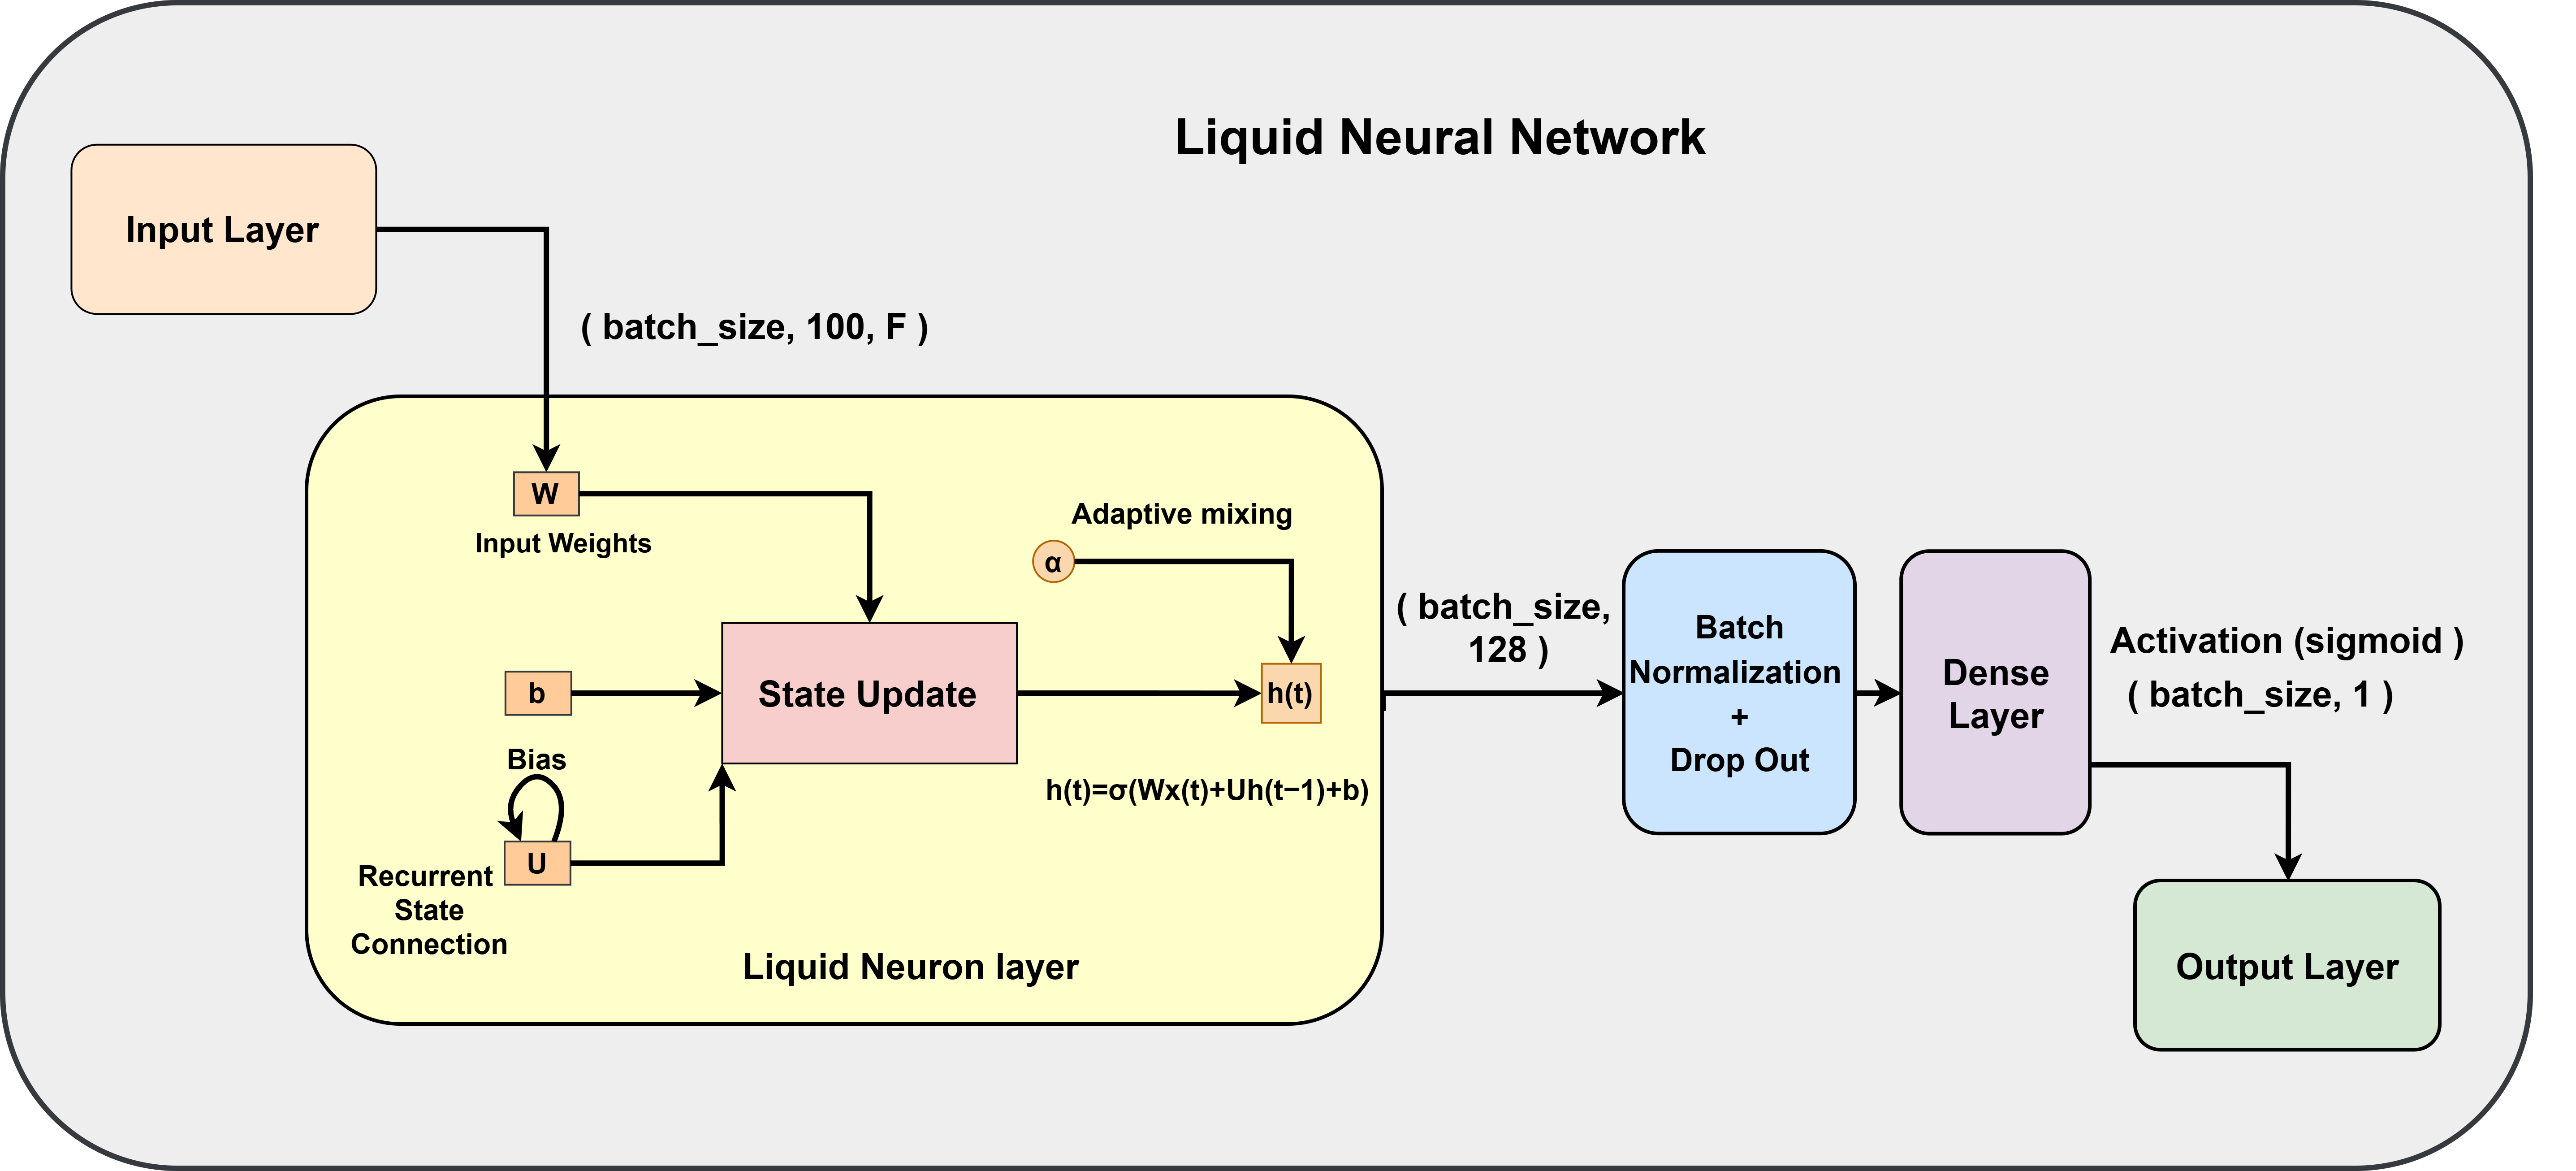
\includegraphics[width=1\textwidth,height=0.5\textwidth]{figures/lnn.png}
\caption{Internal Overview of LNN with Input/Output Dimensions and Activations }\label{Fig2}
\end{figure}


\begin{algorithm}[!ht]
\caption{LNN Model Training and Inference}
\label{algo2}
\DontPrintSemicolon
\KwIn{Input tensor $X \in \mathbb{R}^{128 \times 100 \times F}$, $F \in \{52, 205, 13\}$}
\KwOut{Binary predictions $Y \in \{0,1\}^{128}$}

\vspace{0.1cm}
\textbf{Def ForwardLNN}$(X)$: \tcp*{LNN forward computation}
\Indp
Initialize hidden state $h(0) \leftarrow \vec{0} \in \mathbb{R}^{128}$\;
\For{$t = 1$ \KwTo $100$}{
    Extract time slice $x(t) \in \mathbb{R}^{128 \times F}$ from $X$\;
    Compute hidden update:
    \[
    h(t) = \sigma(Wx(t) + Uh(t-1) + b)
    \]
    Apply adaptive mixing to refine $h(t)$\;
}
$H \leftarrow h(100) \in \mathbb{R}^{128 \times 128}$\;
Apply BatchNorm and Dropout to $H$\;
$Z = \text{Dense}(H) \in \mathbb{R}^{128 \times 1}$\;
$\hat{Y} = \sigma(Z)$ \tcp*{Sigmoid output}
\Indm
\Return{$\hat{Y}$}

\vspace{0.2cm}
\textbf{Def TrainLNN}$(X_{\text{train}}, y_{\text{train}}, X_{\text{val}}, y_{\text{val}})$:\ \\
\Indp
Initialize optimizer (Adam) and loss = \texttt{Weighted BCEWithLogitsLoss}\;
Train up to 100 epochs with batch size 128 and early stopping based on validation loss\;
Save best-performing checkpoint\;
\Indm
\Return{Trained model $f_{\text{LNN}}$}

\vspace{0.2cm}
\textbf{Def TestLNN}$(f_{\text{LNN}}, X_{\text{test}})$:\ \\
\Indp
$\hat{Y} \leftarrow f_{\text{LNN}}(X_{\text{test}})$\;
\For{$i = 1$ \KwTo $128$}{
    $Y_i \leftarrow (\hat{Y}_i \geq 0.5)$ \tcp*{1 = Malicious, 0 = Non-malicious}
}
\Indm
\Return{$Y$}
\end{algorithm}

The core computation is governed by the recurrent update rule:

\begin{equation}\label{eq7}
h(t) = \sigma(Wx(t) + Uh(t-1) + b)
\end{equation}


The input at time step \(t\) is represented by \(x(t) \in \mathbb{R}^F\), the input and recurrent weight matrices are represented by \(W \in \mathbb{R}^{F \times 128}\) and \(U \in \mathbb{R}^{128 \times 128}\), the bias term is represented by \(b \in \mathbb{R}^{128}\), and nonlinearity is introduced by \(\sigma = \tanh\).  To improve temporal adaptivity, a mixing mechanism which dynamically balances the impact of previous hidden states and new inputs, allowing the network to efficiently capture changing behavioral dynamics.






Each of the two stacked recurrent layers that make up the LNN architecture maintains a hidden state with dimensions of 128.  The final hidden representation \(h(100) \in \mathbb{R}^{128 \times 128}\) functions as a compact, temporally-aware embedding of user activity after processing all 100 time steps. This effectively summarizes long-term behavioral dependencies for insider threat classification as shown step by step in Algorithm~\ref{algo2}. Timely insider threat detection is made possible by the LNN's adaptive and recurrent nature, which enables the model to detect minute temporal variations in user behavior.
